\documentclass[a4j]{jarticle}
\usepackage{listings}
\usepackage[dvipdfmx]{graphicx}
\usepackage{here}
\usepackage{ascmac}
\usepackage{comment}


%先生に解説用に使う
%\begin{screen}
%\begin{verbatim}

%\end{verbatim}
%\end{screen}


\begin{document}
%
%表紙の作成
%
\begin{titlepage}
\title{Processingを触ってみよう!}
\author{
\\
立命館大学情報理工学部情報理工学科知能情報コース2回生\\
伊藤聡子 
\\
}
\date{2018年10月19日}
\maketitle
\thispagestyle{empty}
\newpage
\end{titlepage}


%
%Processingについて
%
\section{Processingとプログラミング}
\subsection{Processingの画面説明}
\begin{figure}[h]
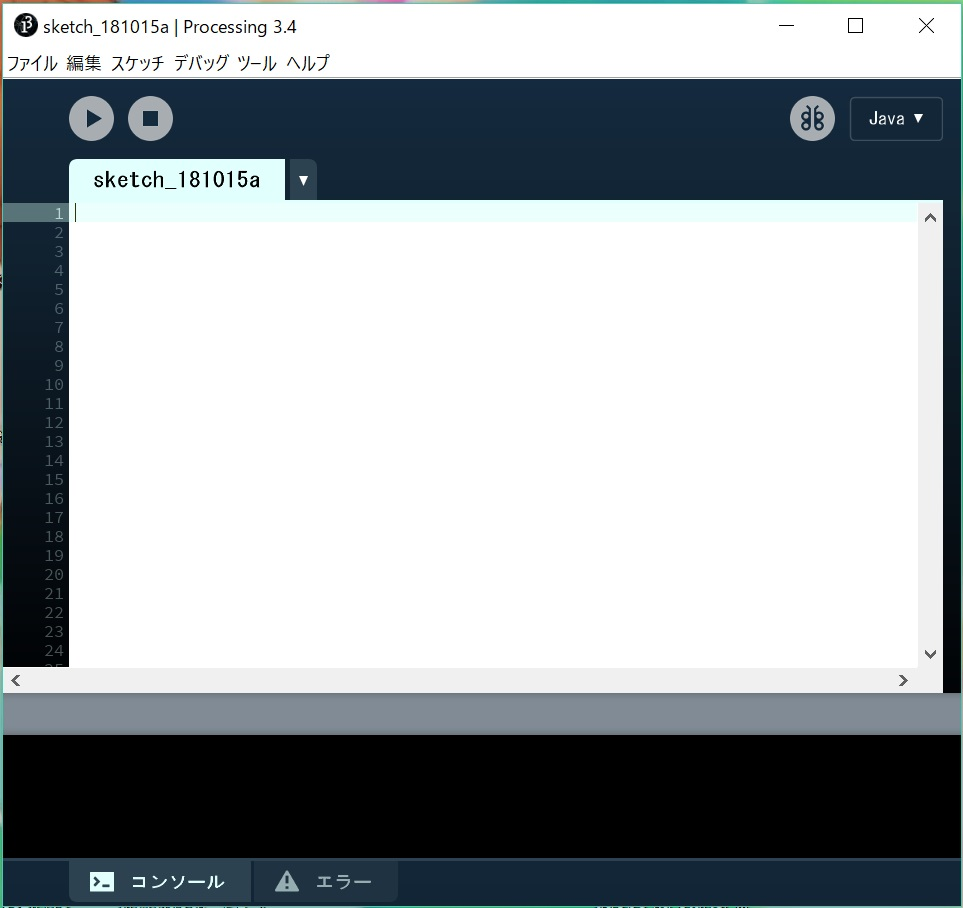
\includegraphics[width=17cm]{processing.JPG}
\end{figure}
\begin{figure}[h]
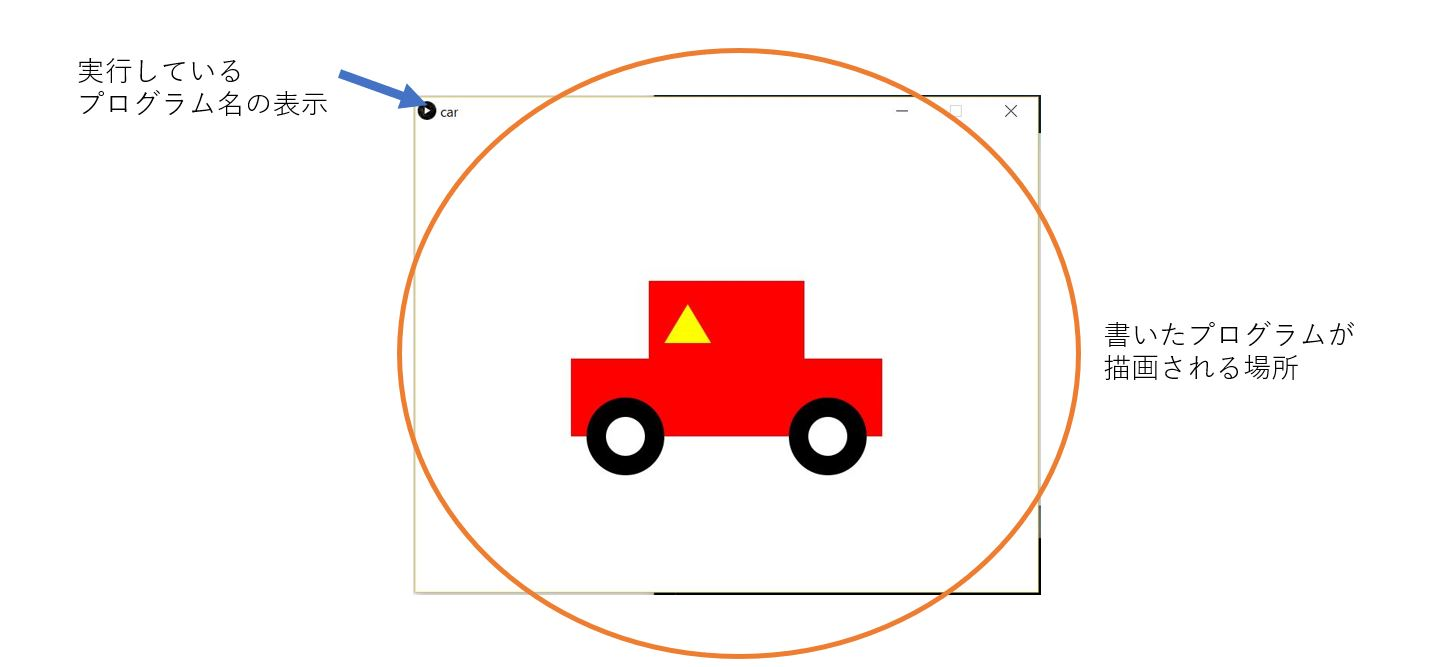
\includegraphics[width=17cm]{ProcessingJ.JPG}
\end{figure}
※プログラミングする際の注意\\
 プログラミングしているとき,エラーが表示されるところが赤色であれば,エラーがある.\\
 そうでなければエラーがない状態.\\
 エラーがない状態になってから,実行ボタンを押す.

\subsection{プログラミングの基礎}
\subsubsection{処理とその流れ}
重要な,覚えておかなければならないことは
\begin{enumerate}
\item プログラムは上から順に処理される
\item 一つ一つの処理の最後には「;」(セミコロン)を付ける
\item エラーがあるときは,実行できない
\end{enumerate}


\subsection{色と形}
\subsubsection{サンプルプログラムを見てみよう}
itosato\_ c2\_ 20181019 > Program > shape\_ and\_ color > shape\_ and\_ color.pdeというファイルを開く.\\
ファイルには,以下のプログラムが書かれている.

\begin{lstlisting}[
	frame=single, 
	basicstyle=\ttfamily, 
	numbers=left, 
	numbersep=8pt, 
	tabsize=2,
	extendedchars=true, 
	xleftmargin=17pt, 
	framexleftmargin=17pt, 
	caption= shape\_ and\_ color]
void setup(){
  size(800, 600); 
}

void draw(){
  background(255, 255, 255);
  noStroke();
  

  fill(0, 0, 0);
  
  ellipse(150, 200, 200, 200);
  
  rect(0, 0, 200, 200);
  
  triangle(650, 100, 550, 300, 750, 300);
  
   
  fill(255, 0, 0);
  ellipse(150, 450, 200, 200);
  
  fill(0, 255, 0);
  rect(300, 350, 200, 200);
  
  fill(0, 0, 255);
  triangle(650, 350, 550, 550, 750, 550);  
}
\end{lstlisting}
どんなことが書かれているのか,予想してみよう.
\\
\\
\\
\\
\\
\\
\\

\subsection{プログラムを実行してみる}
shape\_ and\_ colorを実行する.\\
 図形が6つ出てきたらよい.\\
 自分の予想と,合っていたところ,間違っていたところを見てみよう.

\subsection{色を変えてみよう}
プログラムの中の, fill(num, num, num); の値を自由に変えてみよう.\\
 プログラムを書き換えたら実行しよう.\\
 プログラムのどこを変えたらどのように変化したのか,見てみよう.\\
\\
 次に,ブラウザを開き,「検索またはWebアドレスを入力」というところに,\\
 https://www.colordic.org/ と入力して,検索する.\\
 上のURLを開いたら,色見本が出てくる.好きな色を選んで,RGB値を変えてみよう.\\
 

\subsection{形を変えてみよう}
次に,RGB値以外のところの数値を変えてみよう.\\
\\
 プログラムを書き換えたら実行する.\\
 プログラムをどのように変えたらどのように変化したのか,見てみよう.\\
\\
\\
\\
\\
\\
\\

\subsection{座標}
Processingは,図形を描くときに座標(位置)を決める必要がある.\\
これは,x座標とy座標を指定して決めている.
\begin{figure}[h]
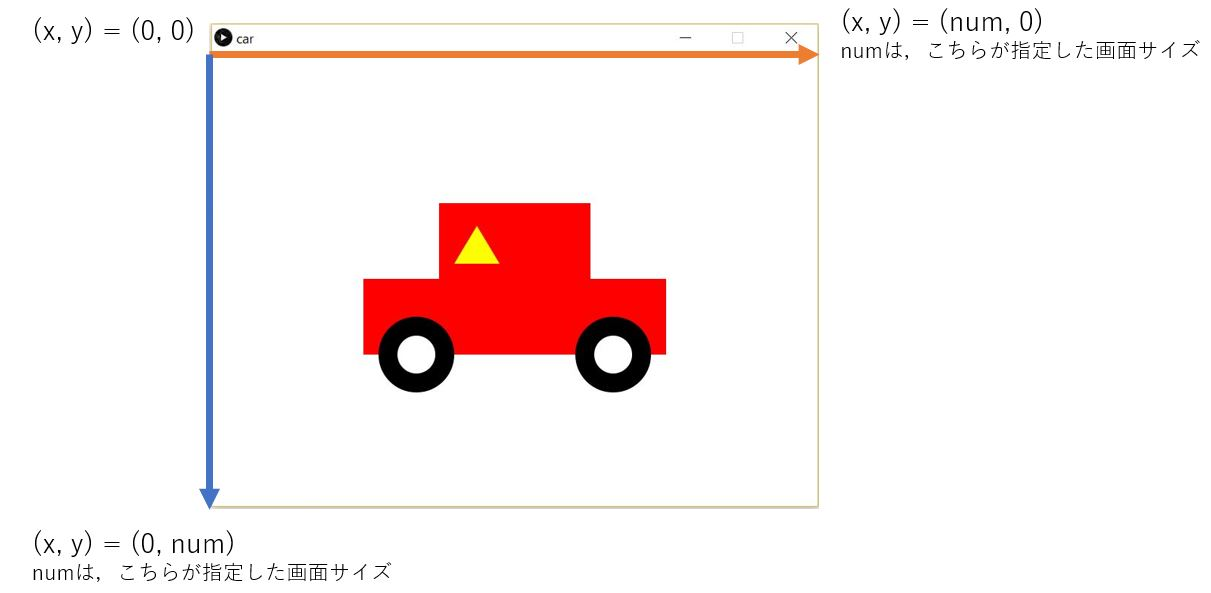
\includegraphics[width=17cm]{zahyou.JPG}
\end{figure}

x軸は右方向に増加する.左上端がx=0.右上端が指定した画面サイズの値となる.\\
 y軸は下方向に増加する.左上端がy=0.左下端が指定した画面サイズの値となる.\\

\subsection{voidと関数}
プログラム中にある「void」とは,関数のこと.ここでいう関数とは,数学の関数とは違い,プログラムの中で処理をまとめたもののことである.\\
関数は,
\begin{screen}
\begin{verbatim}
void 関数名 (){

}
\end{verbatim}
\end{screen}
という風に書く.\\
\{ と\} の間に,実行したいプログラムを書いていく. 
今回の授業の中では,2つの関数を使っている.
\subsubsection{setup}
その名の通り,プログラムを動かすためのセットアップ(準備)をするための関数.\\
ここは,図形を描画するためのキャンバスとなる画面のサイズ指定を行うなどする場所である.

\subsubsection{draw}
その名の通り,描くための関数.\\
この関数の中に図形を描画するためのプログラムを書いていく.

\section{図形を描く}
\subsection{サンプルプログラムを見てみよう}
itosato\_ c2\_ 20181019 > Program > car > car.pde というファイルを開き,プログラムを実行する.

\begin{lstlisting}[
	frame=single, 
	basicstyle=\ttfamily, 
	numbers=left, 
	numbersep=8pt, 
	tabsize=2,
	extendedchars=true, 
	xleftmargin=17pt, 
	framexleftmargin=17pt, 
	caption= car]
void setup(){
 size(800, 600); 
}

void draw(){
  background(255, 255, 255);
  noStroke();
  
  
  fill(255, 0, 0);
  rect(200, 300, 400, 100);
  rect(300, 200, 200, 100);

  fill(0, 0, 0);
  ellipse(270, 400, 100, 100);
  ellipse(530, 400, 100, 100);
  
  fill(255, 255, 255);
  ellipse(270, 400, 50, 50);
  ellipse(530, 400, 50, 50);
  
  fill(255, 255, 0);
  triangle(350, 230, 320, 280, 380, 280);
}
\end{lstlisting}
図形を組み合わせることにより,簡単な絵を描くことが出来る.\\

\subsection{図形の描き方}
ここでは,基本的な図形である,丸,四角,三角の描き方を紹介する.
\subsubsection{丸の描き方}
丸を書くためには,描きたい円の中心座標と縦横の直径を指定する必要がある.\\
具体的には,以下のような書き方をする.
\begin{screen}
\begin{verbatim}
ellipse(中心のx座標, 中心のy座標, 縦の直径, 横の直径);
\end{verbatim}
\end{screen}
横の長さと縦の長さを一緒にすると円が,別にすると楕円を描くことが出来る.
\subsubsection{四角の描き方}
四角を描くためには,左上頂点の座標と,縦横の長さを指定する必要がある.\\
具体的には,以下のような書き方をする.
\begin{screen}
\begin{verbatim}
rect(左上頂点のx座標, 左上頂点のy座標, 横の長さ, 縦の長さ);
\end{verbatim}
\end{screen}
横の長さと縦の長さを一緒にすると正方形が,別にすると長方形を描くことが出来る.

\subsubsection{三角の描き方}
三角を描くには,各頂点の座標を指定する必要がある.\\
具体的には,以下のような書き方をする.
\begin{screen}
\begin{verbatim}
triangle(1つ目の頂点のx座標, 1つ目の頂点のy座標, 2つ目の頂点のx座標, 2つ目の頂点のy座標, 3つ目の頂点のx座標, 3つ目の頂点のy座標);
\end{verbatim}
\end{screen}
各頂点の座標次第では,いびつな形の三角形を描くことが出来る.
\newpage

\section{自由に絵を描く}
\subsection{何を描くか考える}
以下の方眼紙に,絵を下書きしよう.\\
1メモリを10や20で考えるのがいいと思われる.
\begin{figure}[h]
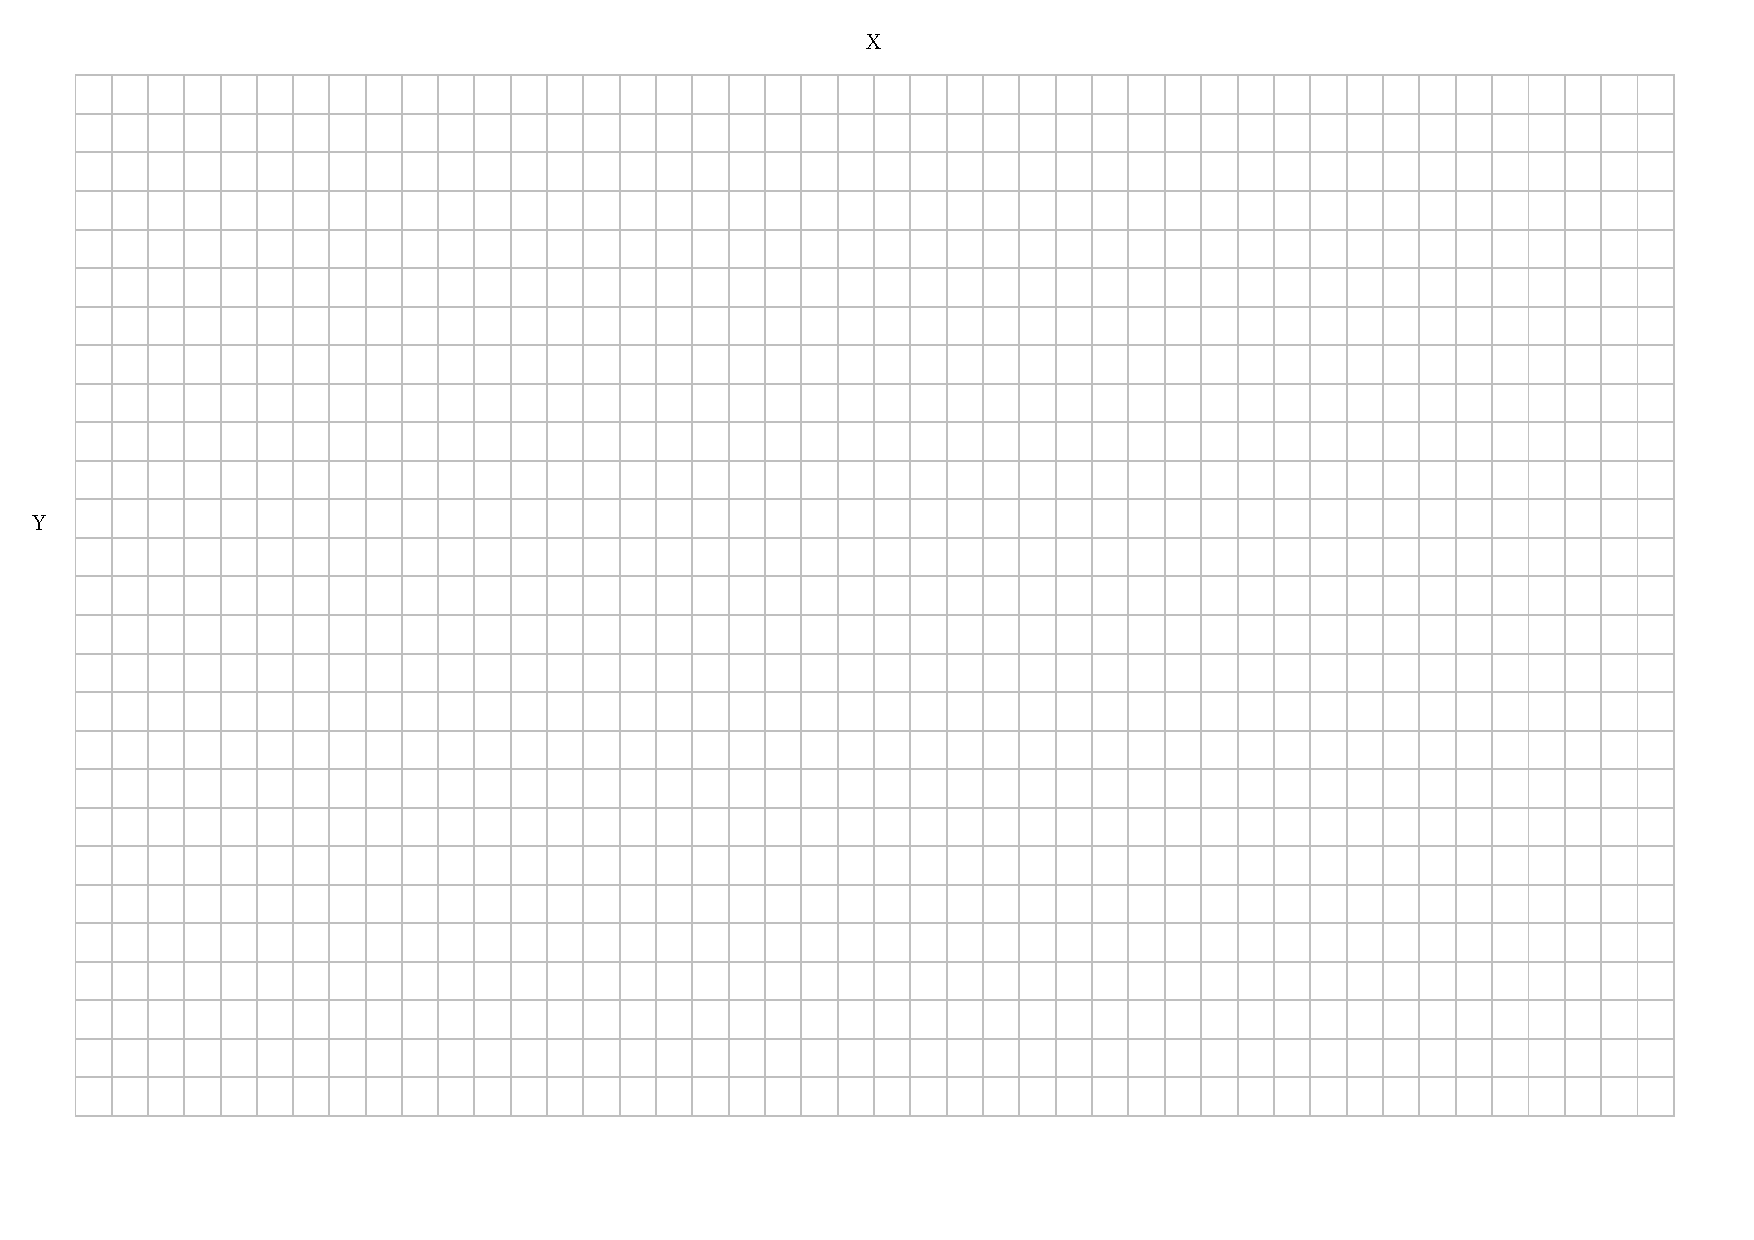
\includegraphics[width=17cm]{hougan.pdf}
\end{figure}
\subsection{どのようなプログラムになるか予想する}
どんなことを書かなければならないのか,自分が分かるようにざっくりとプログラムの流れを書いてみよう.	\\	
最低限考えなければならないのは,
\begin{itemize}
\item どの図形を描くのか
\item どこに図形を描くのか
\item 何色にするのか
\end{itemize}
以上の3点である.

\newpage

\subsection{実際にプログラムを書く}
今までの流れを思い出して,プログラムを書いてみよう!\\
わからなくなったら,手を挙げてすぐに質問しよう.\\
まずは,以下の必ず書かなければならない部分を書いておこう.
\begin{lstlisting}[
	frame=single, 
	basicstyle=\ttfamily, 
	numbers=left, 
	numbersep=8pt, 
	tabsize=2,
	extendedchars=true, 
	xleftmargin=17pt, 
	framexleftmargin=17pt, 
	caption= フォーマット]
void setup(){
  size(num, num); 
}

void draw(){
  background(255, 255, 255);
  noStroke();
  


}
\end{lstlisting}
noStroke(); の下から自由にプログラムを書いていこう.\\
画面サイズは自由に変更しても構わない.
\newpage
\section{教師用コンテンツ}
\subsection{Processingのダウンロード方法}
Processingは無料でダウンロード可能な開発環境となっている.ダウンロードは,\\
https://processing.org/download/ より,自身のPCにあったものをダウンロードする.
ダウンロード後は,zipファイルを解凍し,フォルダを開く.中は以下のような構成となっている.\\
\begin{figure}[h]
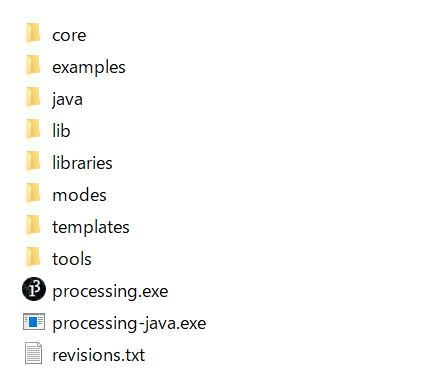
\includegraphics[width=7cm]{t-1.JPG}
\end{figure}
このフォルダの中からはファイルを出さないようにすることに注意する.\\
まずは,processing.exeを開く.すると,以下のような画面が出る.\\
\begin{figure}[h]
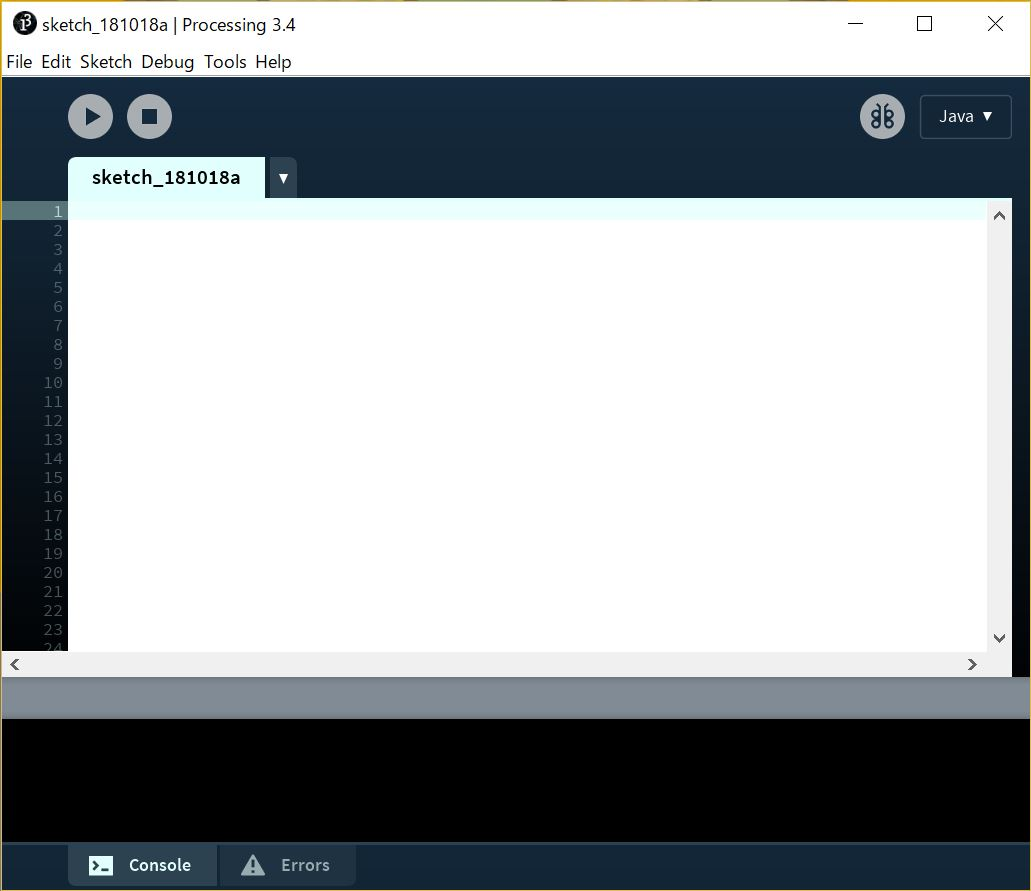
\includegraphics[width=7cm]{t-2.JPG}
\end{figure}
\\
現在の状態でも十分使うことはできるが,次項では日本語に設定するための方法を記す.
\newpage
\subsection{日本語環境の構築}
まず,以下のスクリーンショットのようにPreferencesをクリックする.\\
\begin{figure}[h]
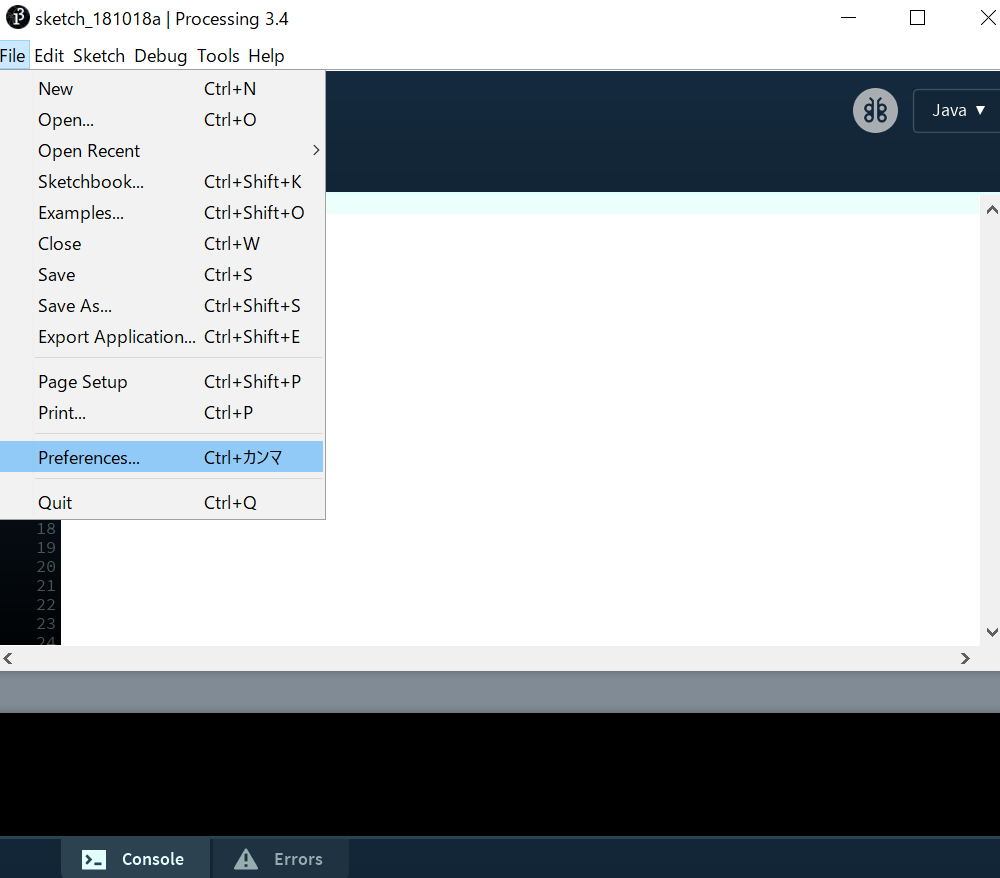
\includegraphics[width=7cm]{t-3.png}
\end{figure}
\\
すると,以下のような画面が現れる.
\begin{figure}[h]
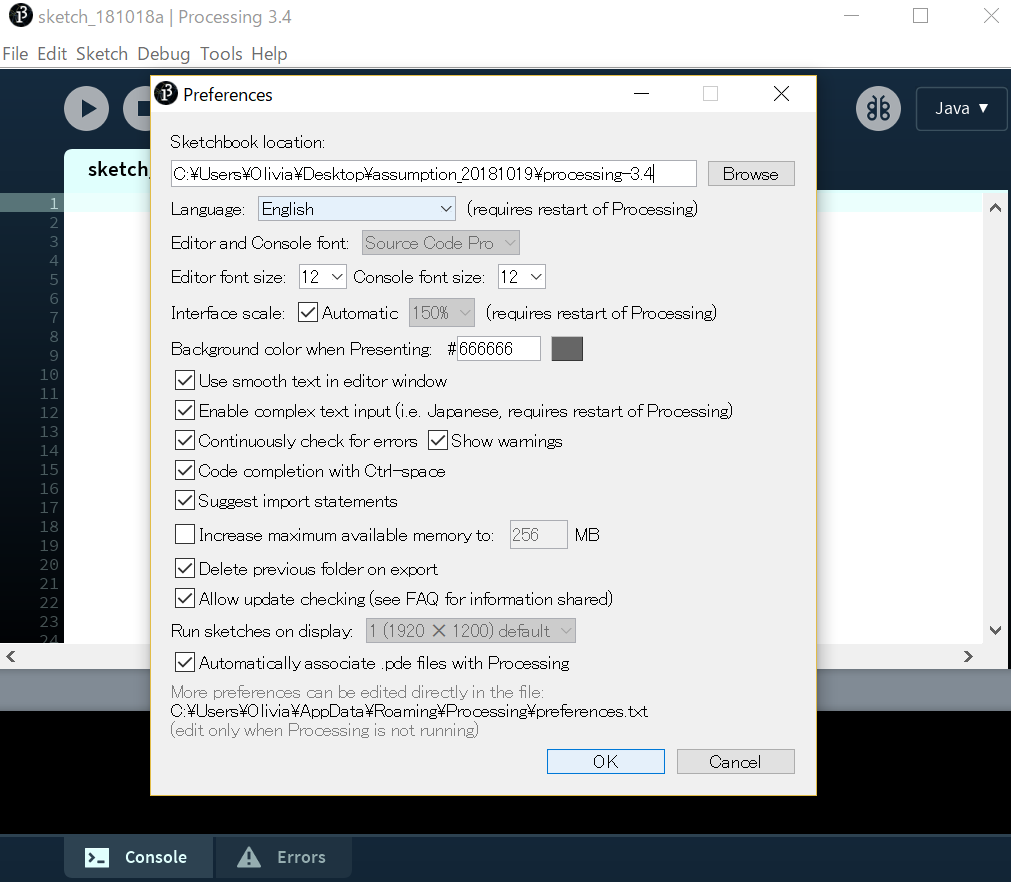
\includegraphics[width=7cm]{t-4.png}
\end{figure}
\\
LanguageをEnglishから日本語に変更し,OKボタンを押す.\\
そして,画面の一番下,詳細な設定は次のファイルを直接編集することで可能です.と書かれているすぐ下のC:\verb#\#Users から始まる部分をクリックする.すると,エクスプローラーが開く.\\
その中のPreferences.txtを開く.そして,editor.font.familyをHG創英角ゴシックUBに変更.\\
全てのウィンドウを閉じる.以上で,日本語の環境を構築できた.日本語でのコメントアウトも官僚となっている.
\subsection{全プログラムの解説}
以下のプログラムには,コメントアウトで解説を加えている.\\
コメントアウトとは,プログラマがプログラムを書く際に,メモ書きや説明文をプログラム内に書き残すことで,よりそのプログラムが分かりやすいものにしている部分のことである.\\
Processingにおいては,コメントアウトしたい部分のはじめに//(ダブルスラッシュ)を付けることにより,その行の最後までをコメントアウトできるようになっている.\\

\subsubsection{shape\_ and\_ colorの解説}
\begin{screen}
\begin{verbatim}
//セットアップ(初期設定)を行う
void setup(){
//図形を出力する画面のサイズを,800×600にする
  size(800, 600); 
}

//図形を描画する
void draw(){
  //背景色をRGBで指定
  background(255, 255, 255);
  //図形に枠線を付けないようにする
  noStroke();
  
  //以下から描く図形の色を指定
  fill(0, 0, 0);
  
  //円を,中心座標(150,200)のところに,縦横200の大きさで描く
  ellipse(150, 200, 200, 200);
  
  //四角を,左上頂点の座標(300, 100)からx方向(右方向)に200,y方向(下方向)に200の大きさで描く
  rect(300, 100, 200, 200);

  //それぞれの頂点座標が(650, 100),(550, 300),(750, 300)の三角を描く
  triangle(650, 100, 550, 300, 750, 300);
  
  //図形を描く色をRGB(255, 0, 0)に変更する
  fill(255, 0, 0);
  //円を,中心座標(150,450)のところに,縦横200の大きさで描く
  ellipse(150, 450, 200, 200);
  
  //図形を描く色をRGB(0, 255, 0)に変更する
  fill(0, 255, 0);
  //四角を,左上頂点の座標(300, 350)からx方向(右方向)に200,y方向(下方向)に200の大きさで描く
  rect(300, 350, 200, 200);
  
  //図形を描く色をRGB(0, 0, 255)に変更する
  fill(0, 0, 255);
  //それぞれの頂点座標が(650, 350),(550, 550),(750, 550)の三角を描く
  triangle(650, 350, 550, 550, 750, 550);
  
}
\end{verbatim}
\end{screen}

\subsubsection{carの解説}
\begin{screen}
\begin{verbatim}
//セットアップ(初期設定)を行う
void setup(){
//図形を出力する画面のサイズを,800×600にする
  size(800, 600); 
}


//図形を描画する
void draw(){
  //背景色をRGBで指定
  background(255, 255, 255);
  //図形に枠線を付けないようにする
  noStroke();
  
  
  //図形を描く色をRGB(255, 0, 0)に変更する
  fill(255, 0, 0);
  //四角を,左上頂点の座標(200, 300)からx方向(右方向)に400,y方向(下方向)に100の大きさで描く
  rect(200, 300, 400, 100);
  //四角を,左上頂点の座標(300, 200)からx方向(右方向)に200,y方向(下方向)に100の大きさで描く
  rect(300, 200, 200, 100);

  //図形を描く色をRGB(0, 0, 0)に変更する
  fill(0, 0, 0);
  //円を,中心座標(270, 400)のところに,縦横100の大きさで描く
  ellipse(270, 400, 100, 100);
  //円を,中心座標(530, 400)のところに,縦横100の大きさで描く
  ellipse(530, 400, 100, 100);
  
  //図形を描く色をRGB(255, 255, 255)に変更する
  fill(255, 255, 255);
  //円を,中心座標(270, 400)のところに,縦横50の大きさで描く
  ellipse(270, 400, 50, 50);
  //円を,中心座標(530, 400)のところに,縦横50の大きさで描く
  ellipse(530, 400, 50, 50);
  
  //図形を描く色をRGB(255, 255, 0)に変更する
  fill(255, 255, 0);
  //それぞれの頂点座標が(350, 230),(320, 280),(380, 280)の三角を描く
  triangle(350, 230, 320, 280, 380, 280);
}
\end{verbatim}
\end{screen}

\end{document}